\chapter{Architecture}

In this section we introduce the general architecture of our wrapper for MonPoly.
A more in depth look at the specific technical implementation will be provided in the implementation section.
In general, we have three components for this project.
On one hand we have the MonPoly with a few extensions.
On the other hand is QuestDB.
Our wrapper acts as the glue between the two.
In addition the wrapper also provides a new interface to MonPoly in the form of a REST API.
Figure \ref{fig:wrapper} shows the structure of the MonPoly wrapper.

% \begin{center}
\begin{figure}
  \centering
  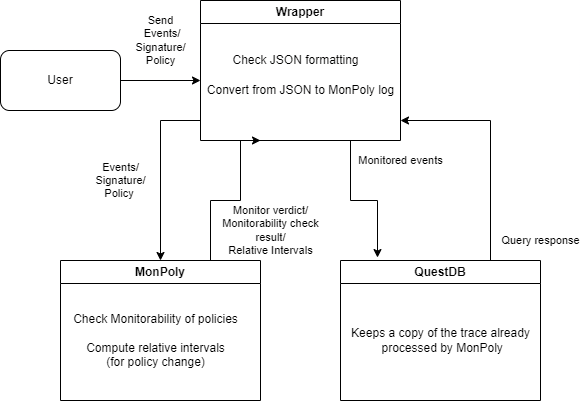
\includegraphics[width=110mm]{diagrams/wrapper.png}
  \caption{Illustration of the project structure}
  \label{fig:wrapper}
\end{figure}

% \end{center}



\section{Wrapper}

The wrapper can be run directly on a system with MonPoly installed.
The alternative and more portable way to run it is with a docker container.
To interact with the wrapper a user can use the provided REST API by sending web requests.

The wrapper runs MonPoly as a subprocess and handles all interactions with MonPoly itself.
Incoming events are first parsed and checked on some major formatting errors.
When the formatting is deemed acceptable the events get forwarded to MonPoly on a per time stamp basis.
If MonPoly reports an issue with a certain time stamp, either it is out of order or one event at that timestamp does not comply with the given signature, this time stamp gets ignored by MonPoly, and in turn the wrapper discards it as well.
If no issue is detected with a timestamp all events in at that timestamp get forwarded to the database.

\section{The REST API}

The interface to the wrapper is a REST API.
We will now introduce the main endpoints and give brief usage examples.






